
% This LaTeX was auto-generated from MATLAB code.
% To make changes, update the MATLAB code and republish this document.

\documentclass{article}
\usepackage{graphicx}
\usepackage{color}

\sloppy
\definecolor{lightgray}{gray}{0.5}
\setlength{\parindent}{0pt}

\begin{document}

    
    
\subsection*{Contents}

\begin{itemize}
\setlength{\itemsep}{-1ex}
   \item Perform regression [1]
   \item MSE
   \item istogrammi
   \item CHIEDERE !!!!!! a\^{} che abbiamo trovato, per trovare la 7esima feature
   \item si fa la combinazione lineare di a\_hat * la riga relativa a un paziente
   \item con tutte le sue features?
   \item the gradient algorithm
   \item istogrammi
   \item steepest descent
\end{itemize}
\begin{verbatim}
close all
clear all
clc

load('updrs.mat')
totalpatients = parkinsonsupdrs(size(parkinsonsupdrs,1),1);
matricepazienti = zeros(1,22);
for k = 1:totalpatients
    patient_matrix = parkinsonsupdrs(find(parkinsonsupdrs(:,1)==k),:);
    patient_matrix(:,4) = abs(fix(patient_matrix(:,4)));
    days_patient = unique(patient_matrix(:,4));
    for i = 1:length(days_patient)
        day = days_patient(i);
        indexes_day = find(patient_matrix(:,4)==day);
        new_matrix = mean(patient_matrix(indexes_day,:),1);
        matricepazienti = [matricepazienti;new_matrix];
    end
end

matricepazienti = matricepazienti(2:end,:);
\end{verbatim}


\subsection*{Perform regression [1]}

\begin{verbatim}
data_train=zeros(1,22);
data_test=zeros(1,22);
for j = 1 : 36
    data_train_mid = matricepazienti(find(matricepazienti(:,1)==j),:);
    data_train = [data_train;data_train_mid];
end
data_train = data_train(2:end,:);

for j = 37 : 42
    data_test_mid = matricepazienti(find(matricepazienti(:,1)==j),:);
    data_test = [data_test;data_test_mid];
end
data_test = data_test(2:end,:);

m_data_train=mean(data_train,1);
v_data_train=var(data_train,1);

for i = 1:size(data_train,1)
    data_train_norm(i, 1:4) = data_train(i, 1:4);
    for z = 5:22
        data_train_norm(i, z) = (data_train(i, z) - m_data_train(z)) / sqrt(v_data_train(z));
    end
end
mean(data_train_norm,1); % verify it is zero mean and va = 1??
var(data_train_norm,1);

for i = 1:size(data_test,1)
    data_test_norm(i, 1:4) = data_test(i, 1:4);
    for z = 5:22
        data_test_norm(i, z) = (data_test(i, z) - m_data_train(z)) / sqrt(v_data_train(z));
    end
end
mean(data_train_norm,1); % verify it is zero mean and va = 1??
var(data_train_norm,1);

% Perform regression [2]
F0 = 7;
y_train=data_train_norm(:,F0); %% feature che elimino e poi vorr? stimare
X_train=data_train_norm;
X_train(:,F0)=[];  %% tutte le feature senza F0

y_test=data_test_norm(:,F0);
X_test=data_test_norm;
X_test(:,F0)=[];
\end{verbatim}


\subsection*{MSE}

\begin{verbatim}
a_hat = inv(X_train(:,5:end).' * X_train(:,5:end)) * X_train(:,5:end).' * y_train; %

% stima valori _ train
y_train_hat = X_train(:,5:end) * a_hat;

figure
plot(y_train_hat)
hold on
plot(y_train, '-r')

% stima valori _ test
y_test_hat = X_test(:,5:end) * a_hat;

figure
plot(y_test_hat)
hold on
plot(y_test, '-r')
\end{verbatim}


\subsection*{istogrammi}

\begin{verbatim}
figure
hist(y_train - y_train_hat, 50)
figure
hist(y_test - y_test_hat, 50) %% dagli istogrammi capiamo che la dist
% degli errori ? circa una gaussiana? a cosa ? dovuto?
\end{verbatim}


\subsection*{CHIEDERE !!!!!! a\^{} che abbiamo trovato, per trovare la 7esima feature}



\subsection*{si fa la combinazione lineare di a\_hat * la riga relativa a un paziente}



\subsection*{con tutte le sue features?}


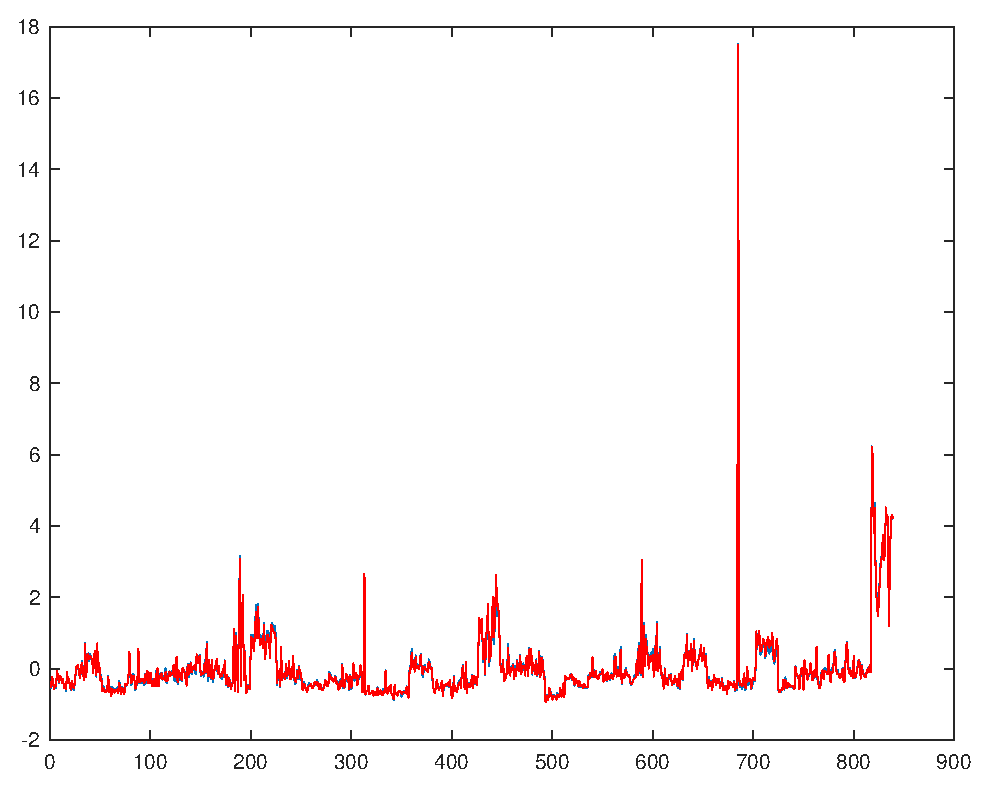
\includegraphics [width=4in]{lab1_01.eps}

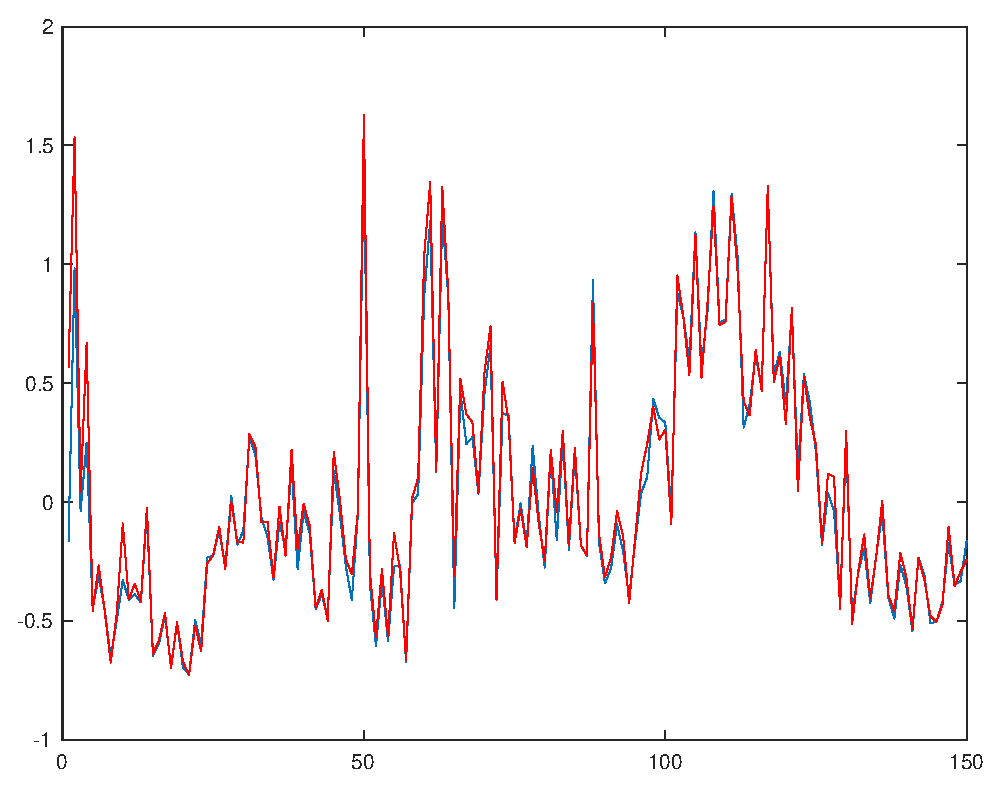
\includegraphics [width=4in]{lab1_02.eps}

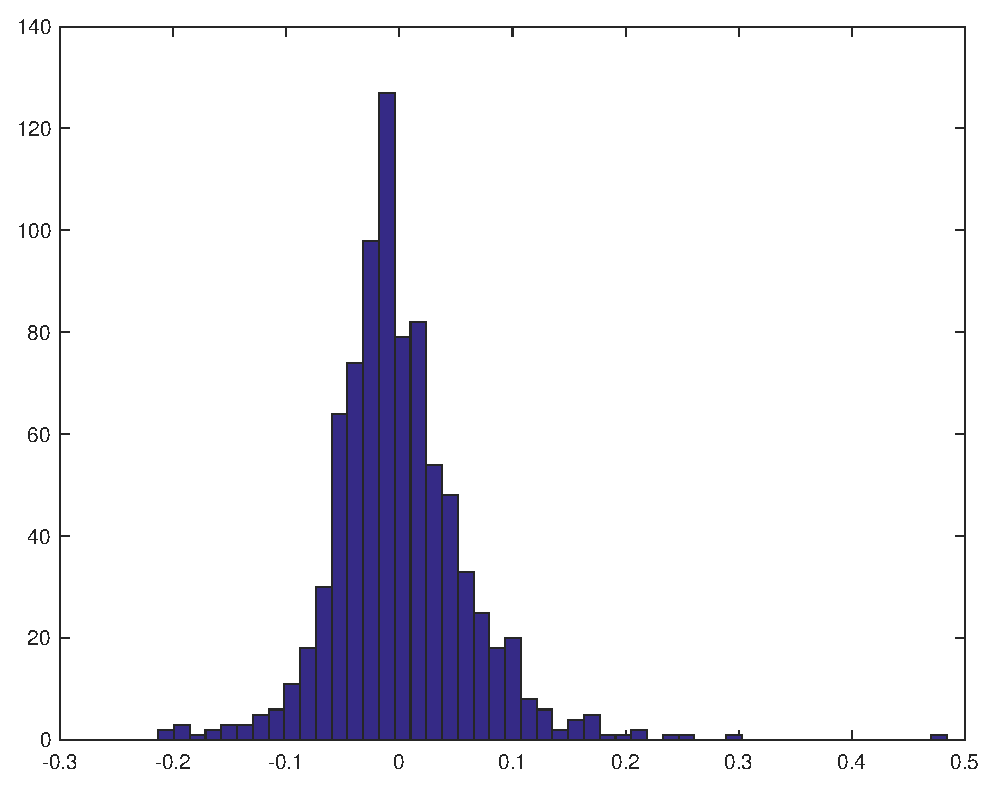
\includegraphics [width=4in]{lab1_03.eps}

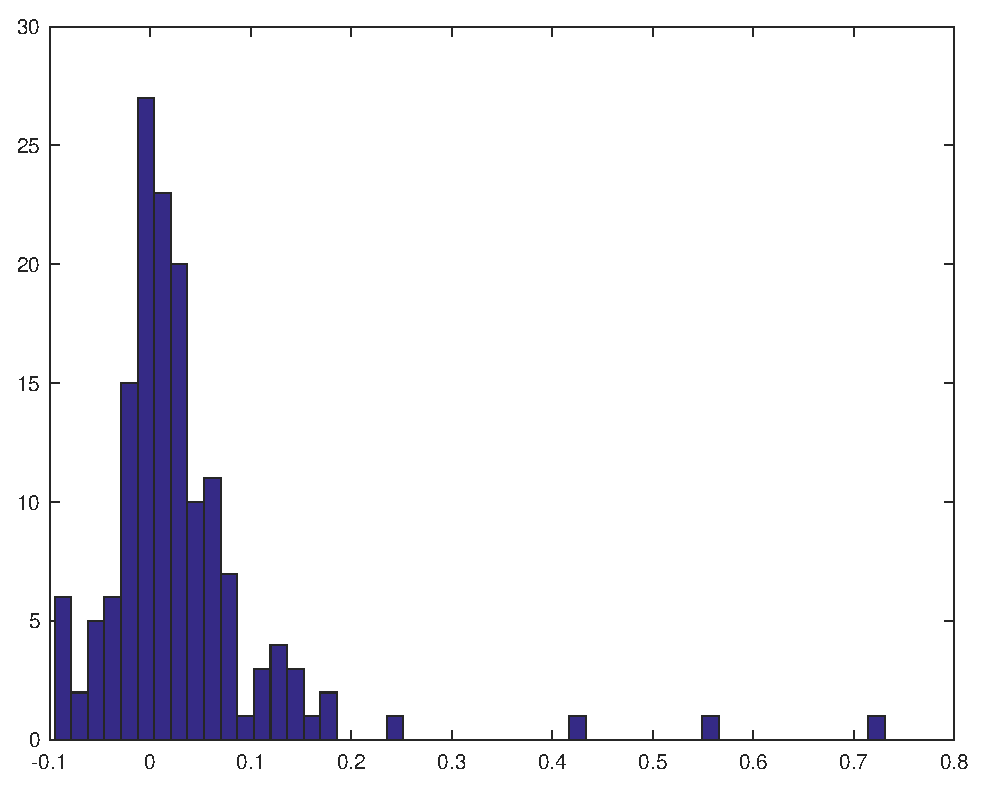
\includegraphics [width=4in]{lab1_04.eps}


\subsection*{the gradient algorithm}

\begin{verbatim}
rng('default')
a_i = rand(17,1);
gamma = 10^-7;
epsilon = 10^-6;
a2 = zeros(17,1);
i=1;

while (norm(a_i - a2) > epsilon)
    grad_a_i = - 2* X_train(:,5:end).' * y_train + 2 * X_train(:,5:end).' * X_train(:,5:end) * a_i;
    a_ii = a_i - (gamma * grad_a_i);
    a2 = a_i;
    a_i = a_ii;
end
a_hat = a_i;

% stima valori _ train
y_train_hat = X_train(:,5:end) * a_hat;

figure
plot(y_train_hat)
hold on
plot(y_train, '-r')

% stima valori _ test
y_test_hat = X_test(:,5:end) * a_hat;

figure
plot(y_test_hat)
hold on
plot(y_test, '-r')
\end{verbatim}


\subsection*{istogrammi}

\begin{verbatim}
figure
hist(y_train - y_train_hat, 50)
figure
hist(y_test - y_test_hat, 50)
\end{verbatim}

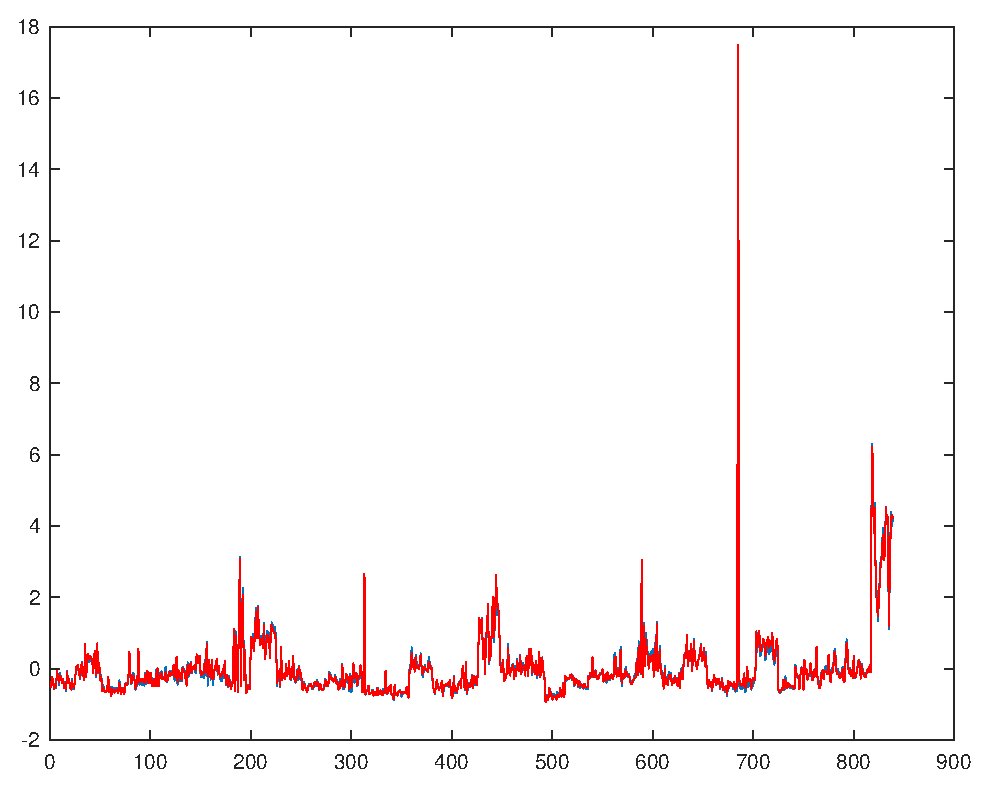
\includegraphics [width=4in]{lab1_05.eps}

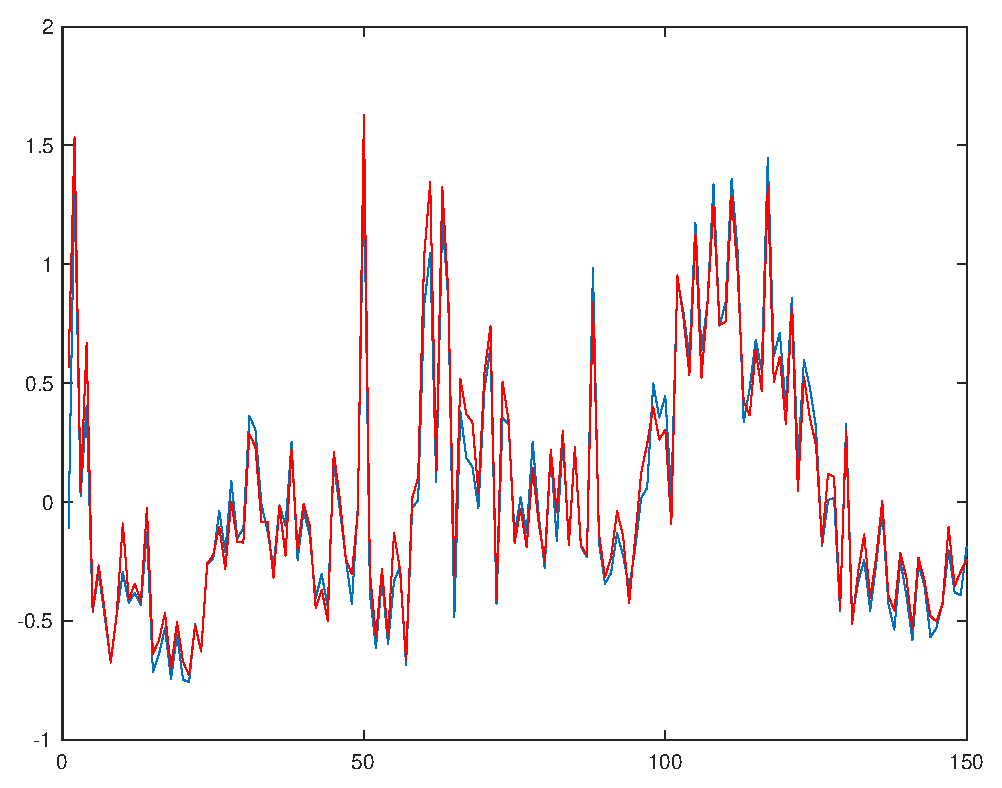
\includegraphics [width=4in]{lab1_06.eps}

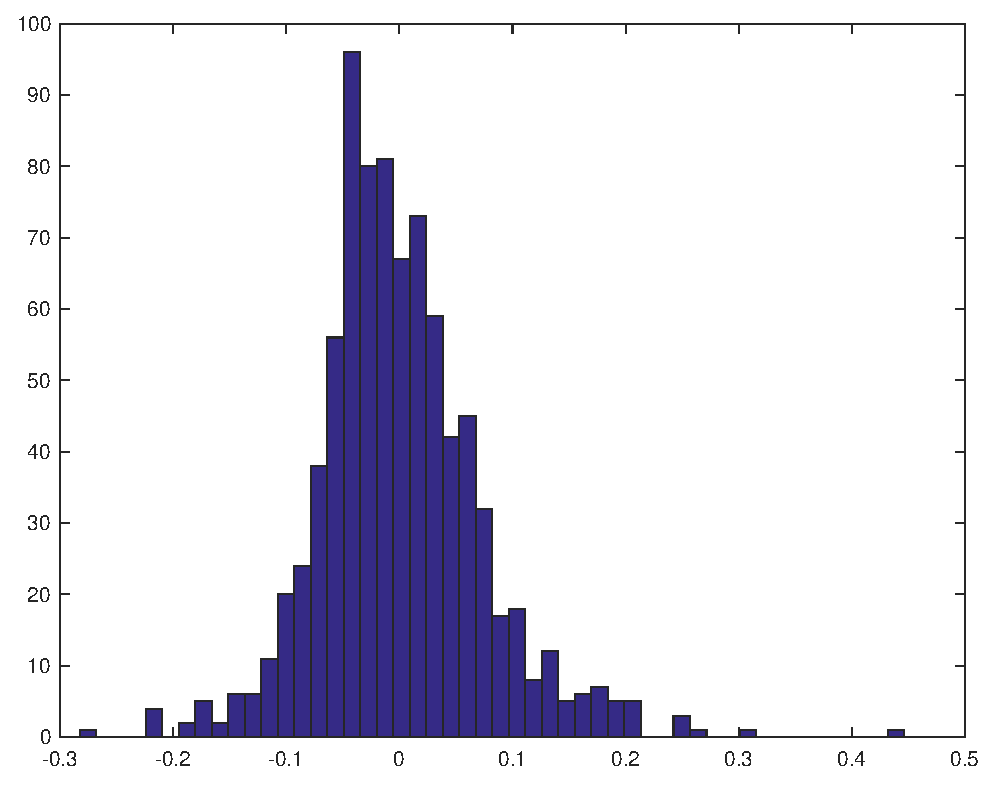
\includegraphics [width=4in]{lab1_07.eps}

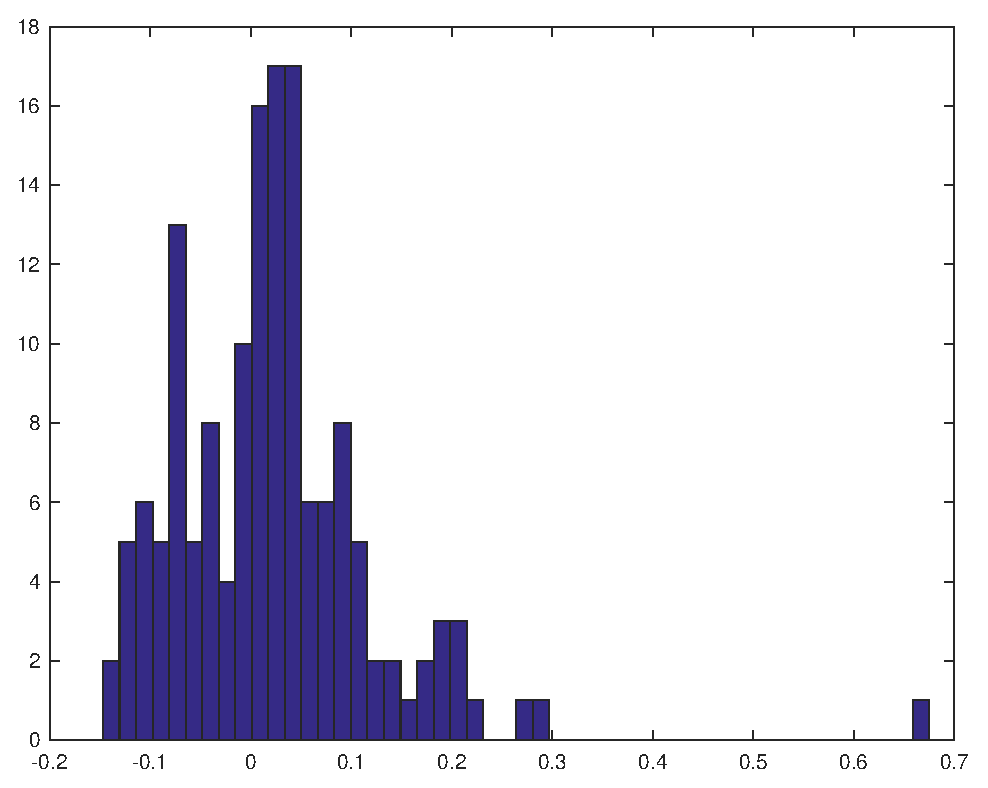
\includegraphics [width=4in]{lab1_08.eps}


\subsection*{steepest descent}

\begin{verbatim}
rng('default')
a_i = rand(17,1);
epsilon = 10^-6;
a2 = zeros(17,1);
i= 1;
while (norm(a_i - a2) > epsilon)
    grad_a_i = - 2* X_train(:,5:end).' * y_train + 2 * X_train(:,5:end).' * X_train(:,5:end) * a_i;
    hess_a_i = 4 * X_train(:,5:end).' * X_train(:,5:end);
    a_ii = a_i - ((norm(grad_a_i)^2 * grad_a_i)/(grad_a_i.' * hess_a_i * grad_a_i));
    a2 = a_i;
    a_i = a_ii;
end
\end{verbatim}



\end{document}
    
